\documentclass[11pt]{article}

\usepackage[margin=1in]{geometry}
\usepackage{graphicx}
\usepackage{booktabs}
\usepackage{hyperref}
\usepackage{amsmath}
\usepackage{authblk}

\title{A Synthetic Exterior Point-Cloud Benchmark for Rockpile Fragmentation and P80 Estimation with EdgeConv Edge Affinity}
\author[1]{Namgyu (Noah) Ha}
\affil[1]{Department of Energy and Resources Engineering, National Korea Maritime and Ocean University, Busan, Republic of Korea}
\date{June 2026}

\begin{document}
\maketitle

\begin{abstract}
Operational fragmentation monitoring increasingly uses photogrammetric or lidar point clouds, but labelled real rockpile scans with point-level fragment identity and independent particle-size-distribution (PSD) ground truth remain scarce. This study presents a reproducible synthetic exterior point-cloud benchmark for rockpile surface clustering and P80 estimation. One hundred no-boundary synthetic rockpile scenes were generated with 150 requested fragments per scene using a physics-informed exterior-surface construction workflow, then split at the scene level into 60 training, 20 validation, and 20 held-out test scenes. A DGCNN-style EdgeConv edge-affinity model was trained to predict whether neighbouring exterior points belong to the same fragment. Connected components of high-affinity edges were converted into surface-cluster PSD proxies, with the edge threshold selected on validation scenes by P80 error and noise-aware post-processing. The model learned edge affinity reliably, reaching validation average precision of 0.9313 at epoch 24. However, downstream PSD estimation remained sensitive to threshold calibration: validation selected the post-split EdgeConv variant at threshold 0.997, and the held-out test mean absolute P80 error was 19.04\% with a mean noise fraction of 0.603. These results indicate that EdgeConv provides a useful controlled benchmark for surface-cluster affinity learning, while robust post-processing and field calibration remain the main barriers to operational P80 estimation.
\end{abstract}

\textbf{Keywords:} rock fragmentation; point cloud; synthetic benchmark; EdgeConv; DGCNN; particle size distribution; P80; photogrammetry; mining

\section{Introduction}
Post-blast fragmentation affects loading, hauling, crushing, and comminution performance. Classical blast-fragmentation models such as Kuz--Ram and Swebrec remain useful because particle size distribution (PSD) links blasting outcomes with mine-to-mill performance \cite{cunningham1983,ouchterlony2005}. Image-based fragmentation systems are widely used, but two-dimensional images must infer scale, occlusion, and particle overlap from a projected surface \cite{palangio1995,siddiqui2009}. Three-dimensional photogrammetry and lidar workflows reduce some of these limitations, but field point clouds rarely include reliable point-level fragment labels \cite{engin2020,onederra2015}.

The practical workflow sought by mine operators is sequential: acquire a rockpile surface, build a local point-cloud graph, infer surface clusters, estimate PSD/P80, and compare the estimate against independent field measurements. The key bottleneck is labelled data. Real rockpile annotation is slow and subjective because of touching fragments, occlusion, dust, shadows, and hidden contacts. Synthetic piles can preserve fragment identity by construction and therefore provide a controlled training and validation stage before field deployment.

This paper reports a compact arXiv-ready benchmark built around that controlled stage. The goal is not to claim field-ready fragmentation measurement. Instead, the benchmark isolates a narrower question: given labelled exterior synthetic rockpile scans, how well can a DGCNN/EdgeConv edge-affinity model learn surface grouping signals, and how does that learning translate into P80 estimates after connected-component post-processing?

\section{Synthetic Exterior Rockpile Dataset}
The reported dataset contains 100 synthetic rockpile scenes. Each scene requested 150 fragments and retained only the exterior point-cloud surface used for learning. The final scene index contains an average of 146.68 visible fragments, 5735.63 exterior points, a mean base radius of 0.898 m, and a mean pile height of 1.084 m. Scenes were split by scene identifier, not by point, into 60 training scenes, 20 validation scenes, and 20 held-out test scenes.

The final production dataset used a no-boundary envelope-relax configuration rather than a full sequential-drop Chrono simulation. During development, full dynamic sequential-drop variants were tested with convex-hull and clump contact. They either required impractical computation for 100 scenes or produced numerical outliers when boundary walls were removed. The production configuration therefore uses a faster DEM-relaxation surrogate that preserves labelled fragment meshes for sampling while producing stable exterior pile morphology for the learning benchmark.

\begin{figure}[t]
\centering
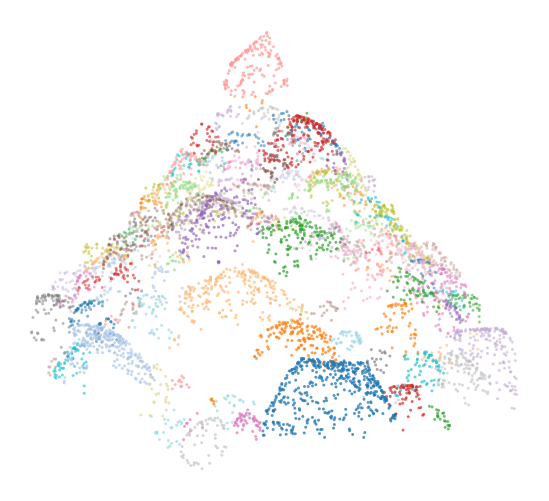
\includegraphics[width=0.82\linewidth]{figures/dem_noboundary_relax150_scene000_preview.png}
\caption{Representative exterior point cloud from the 150-fragment no-boundary synthetic dataset. Colours indicate retained fragment labels on the exterior scan surface.}
\label{fig:scene-preview}
\end{figure}

\section{Edge-Affinity Model}
Fragment identity is scene-specific: fragment 17 in one pile has no semantic relation to fragment 17 in another. The learning problem is therefore formulated as edge affinity. For each local graph edge between neighbouring exterior points, the model predicts whether the two endpoints belong to the same ground-truth fragment.

The model follows the Dynamic Graph CNN/EdgeConv principle of learning local point-cloud features from graph neighbourhoods \cite{wang2019}, in the broader family of point-set learning methods represented by PointNet and PointNet++ \cite{qi2017pointnet,qi2017pointnetpp}. Point features include normalized coordinates, normals, and curvature; edge attributes include geometric differences and local surface cues. During training, a balanced subset of positive and negative edges is sampled from each scene. Photogrammetry-realism augmentation perturbs point positions, normals, curvature, and edge geometry while preserving graph labels, approximating common SfM/MVS imperfections without changing the held-out test labels.

\section{PSD Proxy and Post-Processing}
At inference time, predicted edge probabilities are thresholded. Retained edges define connected components, and each component is interpreted as a visible surface cluster. The cluster is not assumed to be a clean full fragment instance. Instead, it is converted into a PSD proxy using a surface-cluster diameter estimate and an equivalent proxy volume. The volume-weighted cumulative PSD then yields P80.

Four prediction variants are evaluated: raw EdgeConv components, absorbed components where unlabelled points are reassigned by edge affinity, height-marker post-splitting of oversized clusters, and the combined absorb-plus-post-split variant. Thresholds are swept on the 20 validation scenes. The selected setting minimizes a noise-aware validation score while respecting a maximum mean noise fraction where possible.

\section{Training and Validation Results}
The EdgeConv model was trained for 24 epochs with 60 training scenes. Validation metrics were computed on 12 validation scenes per epoch for efficiency. The model learned edge affinity consistently: training loss decreased from 0.5722 to 0.3479, while validation average precision increased from 0.8569 to 0.9313. Validation ROC-AUC reached 0.9179 at epoch 24.

\begin{figure}[t]
\centering
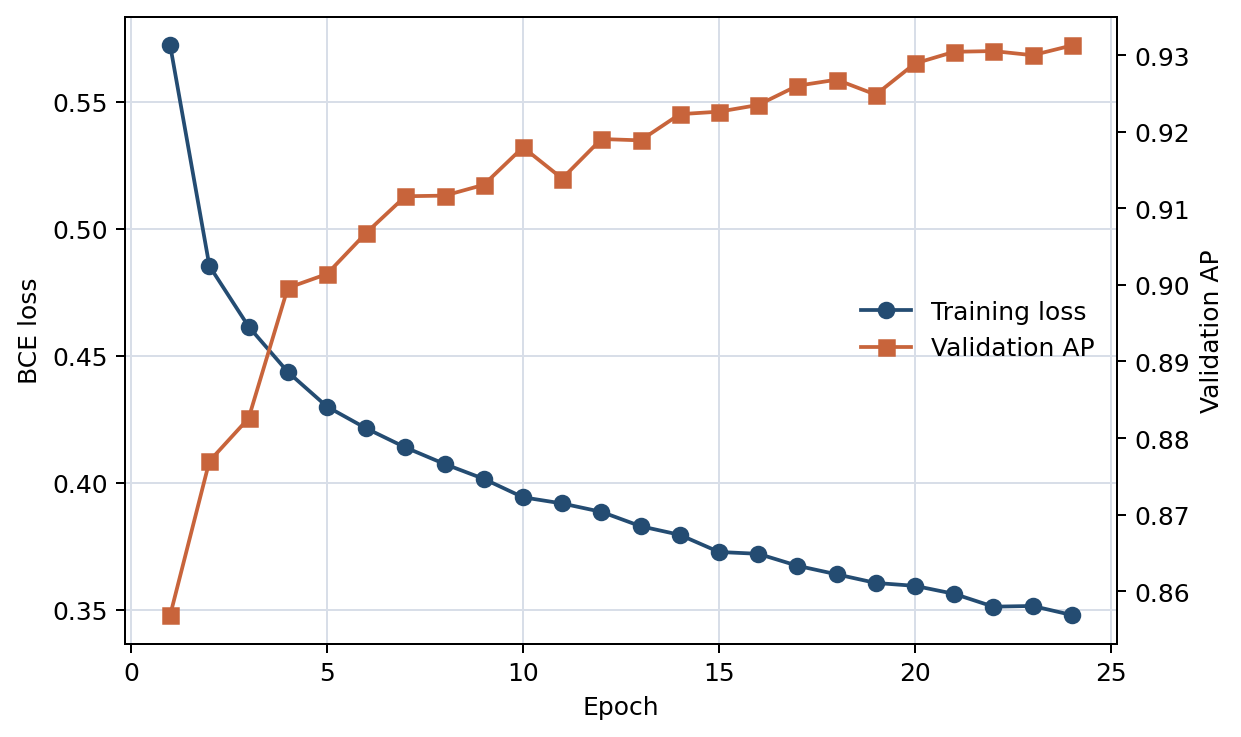
\includegraphics[width=0.78\linewidth]{figures/02_edgeconv_training_curve.png}
\caption{Training loss and validation average precision for the 24-epoch EdgeConv edge-affinity run on the 100-scene no-boundary synthetic dataset.}
\label{fig:training}
\end{figure}

Validation threshold selection showed the main failure mode. Lower thresholds improve component connectivity but merge neighbouring fragments; higher thresholds reduce merging but split many points into small or unlabelled components. The selected operating point was the post-split EdgeConv variant at threshold 0.997. The high threshold indicates that edge probability calibration and connected-component post-processing remain central limitations.

\section{Held-Out Test Results}
The selected validation setting was frozen and evaluated on the 20 held-out test scenes. Table \ref{tab:test-summary} summarizes the four evaluated post-processing variants. The selected post-split EdgeConv variant achieved a mean absolute P80 error of 19.04\% and a median absolute P80 error of 18.36\%. The raw EdgeConv variant gave 20.82\% mean absolute P80 error. Absorption reduced noise fraction from about 0.60 to about 0.51 but worsened P80 error in this run.

\begin{table}[t]
\centering
\caption{Held-out test summary for the 20 test scenes.}
\label{tab:test-summary}
\begin{tabular}{lrrrr}
\toprule
Variant & Threshold & Mean abs. P80 error (\%) & Median abs. P80 error (\%) & Mean noise fraction \\
\midrule
EdgeConv post split & 0.997 & 19.04 & 18.36 & 0.603 \\
EdgeConv raw & 0.997 & 20.82 & 19.42 & 0.603 \\
EdgeConv absorb + post split & 0.997 & 21.84 & 21.40 & 0.506 \\
EdgeConv absorb & 0.997 & 23.45 & 21.40 & 0.506 \\
\bottomrule
\end{tabular}
\end{table}

\begin{figure}[t]
\centering
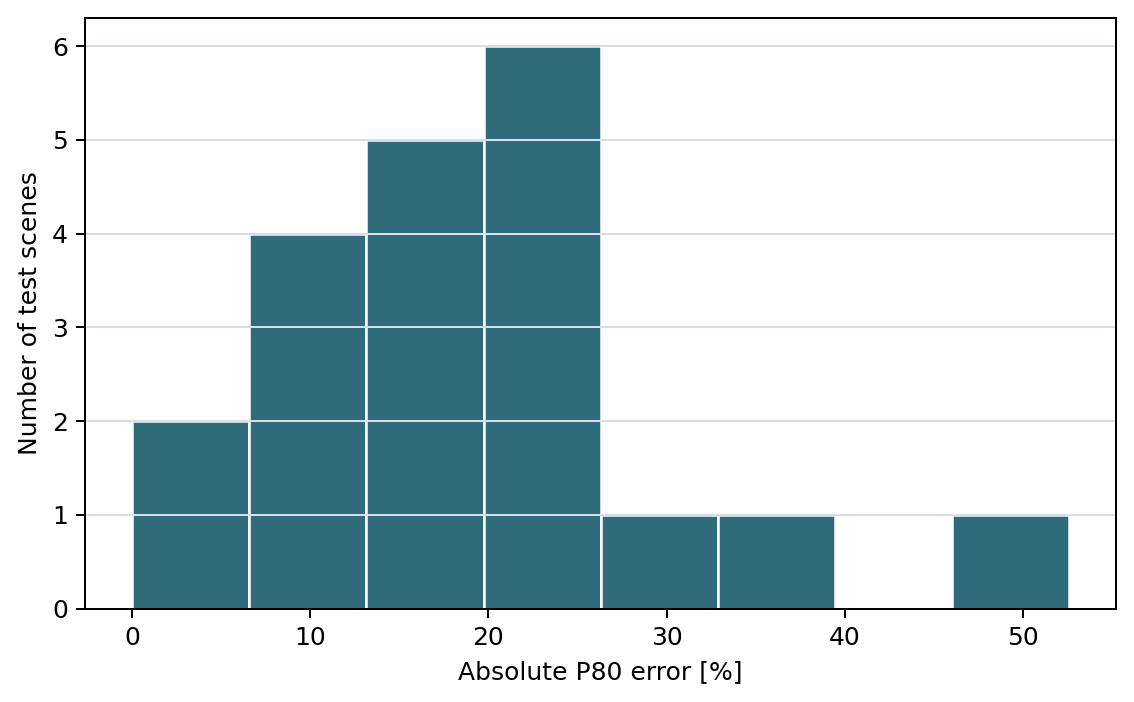
\includegraphics[width=0.70\linewidth]{figures/03_edgeconv_test_p80_error_histogram.png}
\caption{Held-out test distribution of absolute P80 error for the validation-selected EdgeConv post-split setting.}
\label{fig:p80-hist}
\end{figure}

\section{Discussion}
The results are clear but modest. The network learns edge affinity: validation AP improves steadily across 24 epochs and reaches 0.9313. The downstream PSD result is weaker because thresholded connected components are brittle. The validation procedure selected a very high edge threshold, 0.997, and the held-out noise fraction remained approximately 60\%. This behaviour matches earlier realistic-DEM trials: the learning problem is not simply failing, but the mapping from edge probabilities to clean PSD-relevant components is under-calibrated.

The no-boundary 150-fragment dataset is more stable than the attempted sequential-drop Chrono scenes and is practical for 100-scene training. Nevertheless, it is still synthetic and still uses a surface-cluster PSD proxy. Real muckpile deployment requires independent field PSD references and a frozen, pre-specified calibration protocol. Future work should therefore focus on threshold calibration, noise-aware merging rules, learned graph partitioning beyond a single hard threshold, and validation against real photogrammetry or lidar scans.

\section{Reproducibility}
The repository accompanying this manuscript includes the scene index, summary CSV files, training script, evaluation script, figures, and manuscript source. The full generated `.npz` scenes and model checkpoint are treated as regenerated artifacts rather than committed source files. The reported run used 100 scenes, a 60/20/20 scene-level split, 24 training epochs, 22,000 maximum training edges per scene, 36,000 maximum validation edges per scene, and photogrammetry-realism augmentation strength 0.75.

\section{Conclusion}
This benchmark shows that EdgeConv edge affinity can learn useful local surface relationships in labelled synthetic rockpile exterior scans. The best validation AP reached 0.9313, but the held-out mean absolute P80 error remained 19.04\% under a high-threshold post-split connected-component rule. The main research bottleneck is therefore no longer only synthetic data generation or edge-affinity learning; it is robust calibration from edge probabilities to PSD-relevant components. The dataset and code provide a reproducible baseline for that next step.

\section*{Acknowledgments}
During preparation of this manuscript, the author used OpenAI Codex for drafting, coding, formatting, and reproducibility assistance. The author reviewed and edited the output and takes responsibility for the manuscript.

\section*{Data and Code Availability}
Code, manuscript source, figures, and summary tables are prepared for release at \url{https://github.com/Linkgyu/rockpile-edgeconv-arxiv}. The full generated scenes can be regenerated using the included scripts.

\begin{thebibliography}{30}
\bibitem{cunningham1983} Cunningham, C. V. B. The Kuz-Ram model for prediction of fragmentation from blasting. In \emph{Proceedings of the 1st International Symposium on Rock Fragmentation by Blasting}, Lulea, Sweden, 1983.
\bibitem{ouchterlony2005} Ouchterlony, F. The Swebrec function: linking fragmentation by blasting and crushing. \emph{Mining Technology} 2005, 114, 29--44.
\bibitem{palangio1995} Palangio, T. C.; Franklin, J. A.; Maerz, N. H. WIPFRAG: a breakthrough in fragmentation measurement. In \emph{Proceedings of the 21st Annual Conference on Explosives and Blasting Technique}, 1995.
\bibitem{siddiqui2009} Siddiqui, F. I.; Shah, S. M. A.; Behan, M. Y. Measurement of size distribution of blasted rock using digital image processing. \emph{Journal of King Abdulaziz University: Engineering Sciences} 2009, 20, 81--93.
\bibitem{engin2020} Engin, I. C.; Maerz, N. H.; Boyko, K. J.; Reals, R. Practical measurement of size distribution of blasted rocks using LiDAR scan data. \emph{Rock Mechanics and Rock Engineering} 2020, 53, 4653--4671.
\bibitem{onederra2015} Onederra, I.; Thurley, M. J.; Catalan, A. Measuring blast fragmentation at Esperanza mine using high-resolution 3D laser scanning. \emph{Mining Technology} 2015, 124, 34--36.
\bibitem{wang2019} Wang, Y.; Sun, Y.; Liu, Z.; Sarma, S. E.; Bronstein, M. M.; Solomon, J. M. Dynamic Graph CNN for learning on point clouds. \emph{ACM Transactions on Graphics} 2019, 38, 146.
\bibitem{qi2017pointnet} Qi, C. R.; Su, H.; Mo, K.; Guibas, L. J. PointNet: Deep learning on point sets for 3D classification and segmentation. In \emph{Proceedings of CVPR}, 2017.
\bibitem{qi2017pointnetpp} Qi, C. R.; Yi, L.; Su, H.; Guibas, L. J. PointNet++: Deep hierarchical feature learning on point sets in a metric space. In \emph{Advances in Neural Information Processing Systems}, 2017.
\bibitem{ester1996} Ester, M.; Kriegel, H.-P.; Sander, J.; Xu, X. A density-based algorithm for discovering clusters in large spatial databases with noise. In \emph{Proceedings of KDD}, 1996.
\bibitem{pedregosa2011} Pedregosa, F. et al. Scikit-learn: Machine learning in Python. \emph{Journal of Machine Learning Research} 2011, 12, 2825--2830.
\bibitem{paszke2019} Paszke, A. et al. PyTorch: An imperative style, high-performance deep learning library. In \emph{Advances in Neural Information Processing Systems}, 2019.
\end{thebibliography}

\end{document}

